\documentclass[11pt]{beamer}
\usepackage{graphicx}
\usetheme{Warsaw}

\title{\textbf{Hasil Terbaik Konversi chm ke pdf dengan Calibre 0.8.57}}
\subtitle{Contoh kasus: Langkah-langkah mengkonversi ebook (chm) Harun Yahya}
\author{Indra Ginanjar \textless indraginanjar@gmail.com\textgreater }
\date{}
\begin{document}

\begin{frame}
\maketitle
\centering{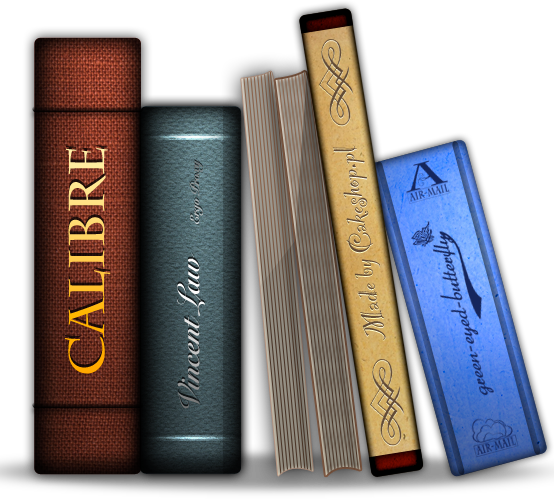
\includegraphics[width=\paperwidth]{graphic/library.png}}
\end{frame}

\begin{frame}
\centering{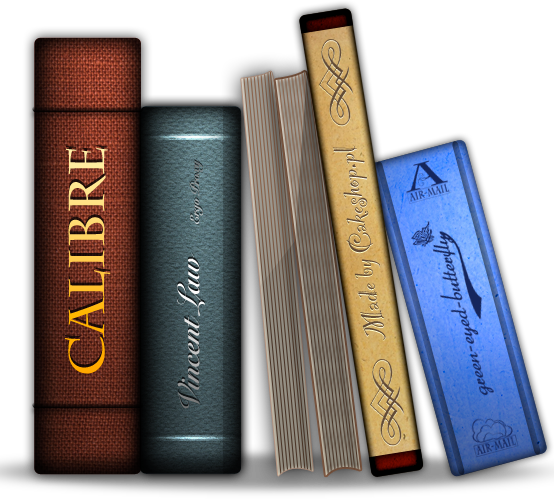
\includegraphics[width=\paperwidth]{graphic/library.png}}
\end{frame}

\begin{frame}
\frametitle{Mengapa 0.8.57 (atau yang lebih baru)?}
\begin{itemize}
\item Versi 0.8.57 mengandung perbaikan hasil konversi ke pdf, teks tidak lagi terpotong pada pergantian halaman 
\item Jika hanya memiliki versi sebelumnya, saran saya:
\begin{enumerate}
\item konversi ke .htmlz (html zip)
\item ekstrak
\item buka dengan firefox
\item print to file (pdf) 
\end{enumerate}
\end{itemize}       
\end{frame}


\begin{frame}[shrink=20]
\frametitle{Contoh hasil koversi ke pdf pada calibre versi sebelumnya}
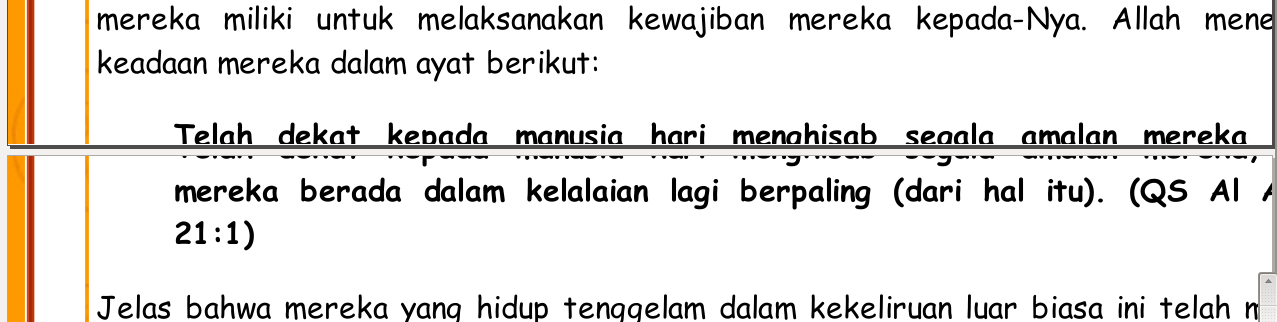
\includegraphics[width=\paperwidth]{graphic/prev_version.png}
\end{frame}

\begin{frame}
\frametitle{Ringkasan langkah-langkah mengkonversi chm ke pdf}
\begin{enumerate}
\item Masukkan chm yang akan dikonversi ke library calibre
\item Pilih bukunya, lalu klik kanan pilih 'Convert Books'
\item Pilih 'pdf' sebagai output format 
\item Centang 'disable font size rescaling'
\item Pilih ukuran kertasnya
\item Pilih 'Default output profile'
\end{enumerate}      
\end{frame}

\begin{frame}[shrink=20]
\frametitle{Masukkan chm yang akan dikonversi ke library calibre}
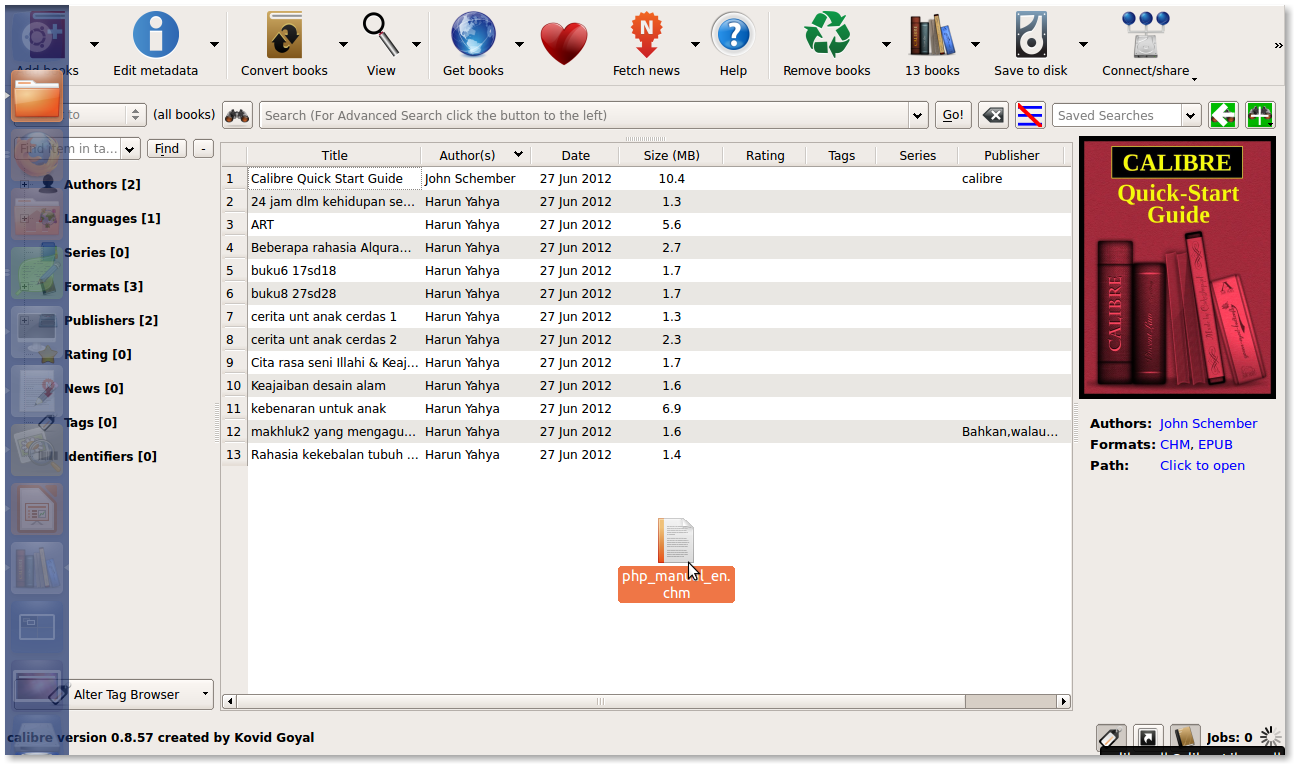
\includegraphics[width=\paperwidth]{graphic/insert_chm.png}
\end{frame}


\begin{frame}[shrink=20]
\frametitle{Pilih bukunya, lalu klik kanan pilih 'Convert Books'}
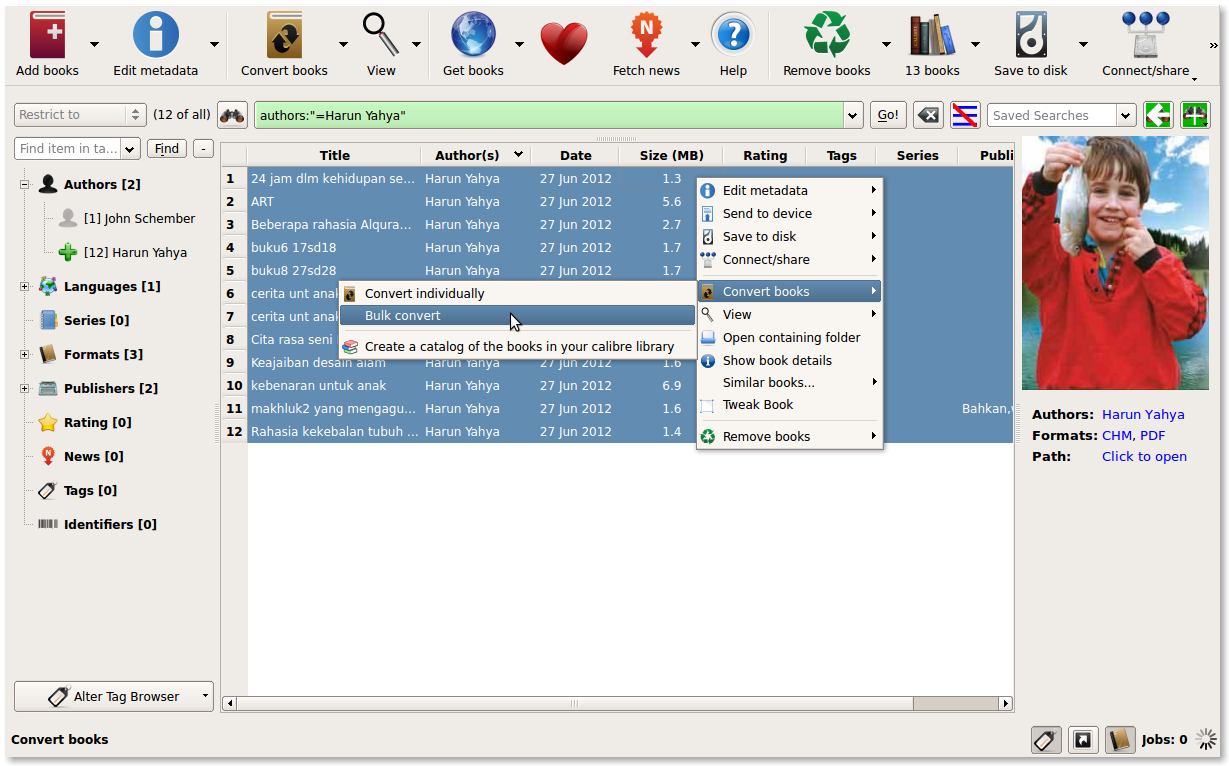
\includegraphics[width=\paperwidth]{graphic/convert_books.png}
\end{frame}

\begin{frame}
\frametitle{Convert books}
\begin{itemize}
\item Konversi bisa dilakukan sekaligus atau satu-persatu
\item Convert individually: tiap buku di konversi dengan pengaturannya masing-masing
\item Bulk convert: semua buku di konversi dengan satu pengaturan
\end{itemize}
\end{frame}

\begin{frame}[shrink=20]
\frametitle{Pilih 'pdf' sebagai output format}
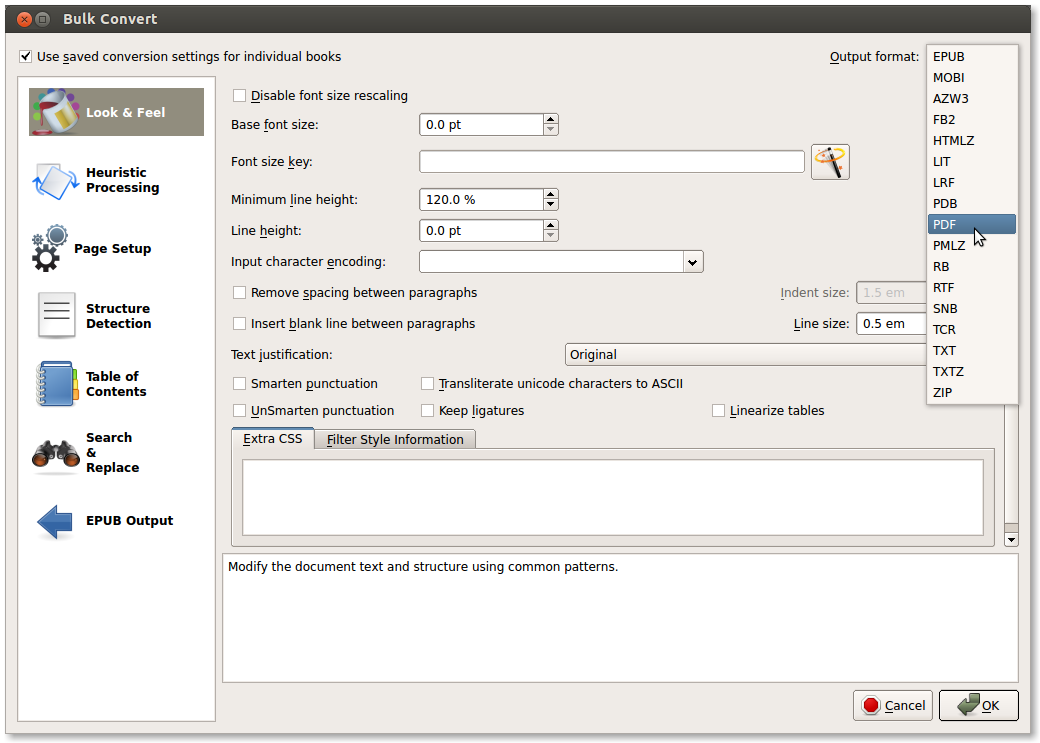
\includegraphics[width=\paperwidth]{graphic/choose_pdf.png}
\end{frame}


\begin{frame}[shrink=20]
\frametitle{Centang 'disable font size rescaling'}
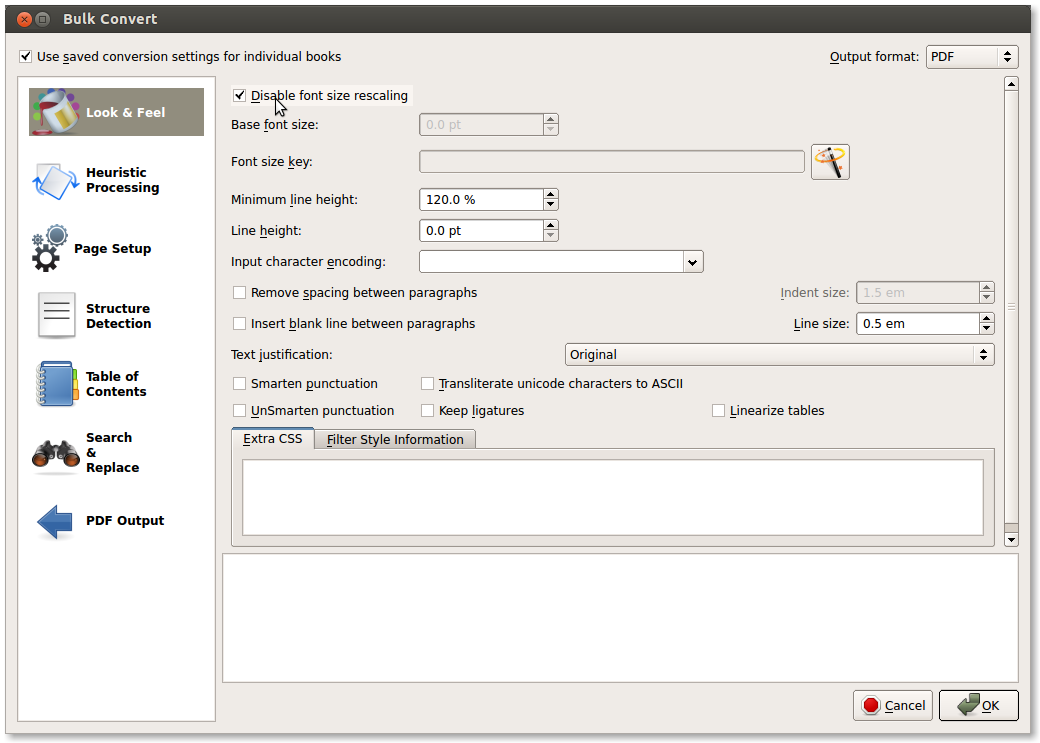
\includegraphics[width=\paperwidth]{graphic/disable_rescaling.png}
\end{frame}


\begin{frame}[shrink]
\frametitle{Pilih ukuran kertasnya}
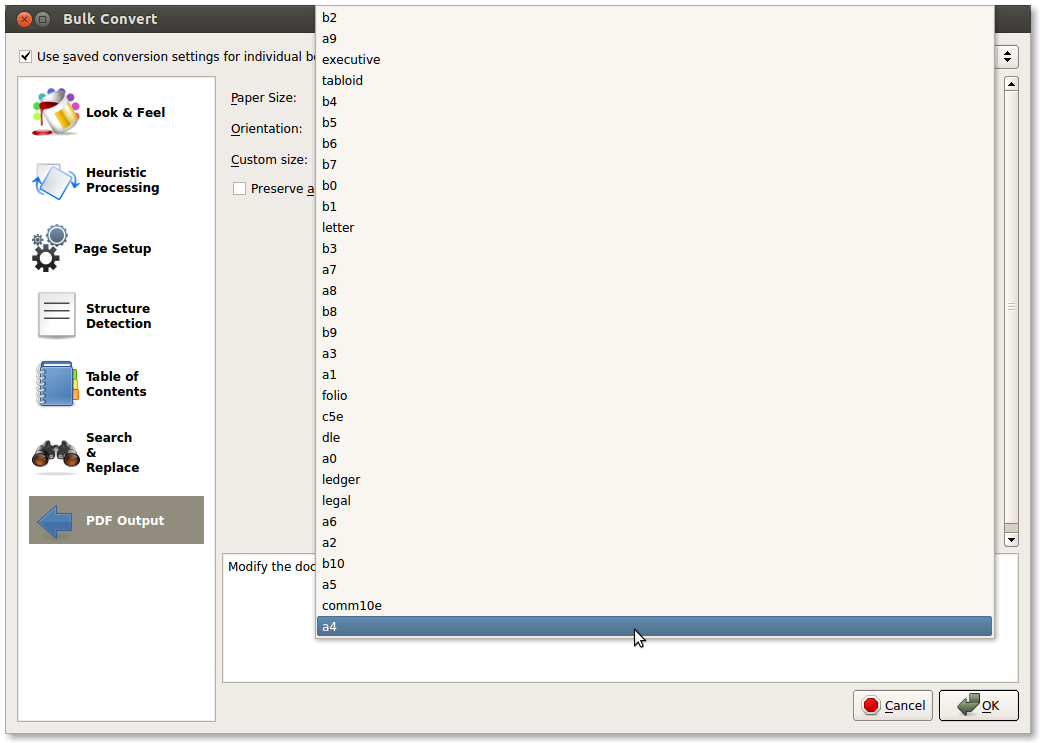
\includegraphics[width=\paperwidth]{graphic/choose_paper.png}
\end{frame}


\begin{frame}[shrink=20]
\frametitle{Penting, lakukan belakangan! Pilih 'Default output profile'}
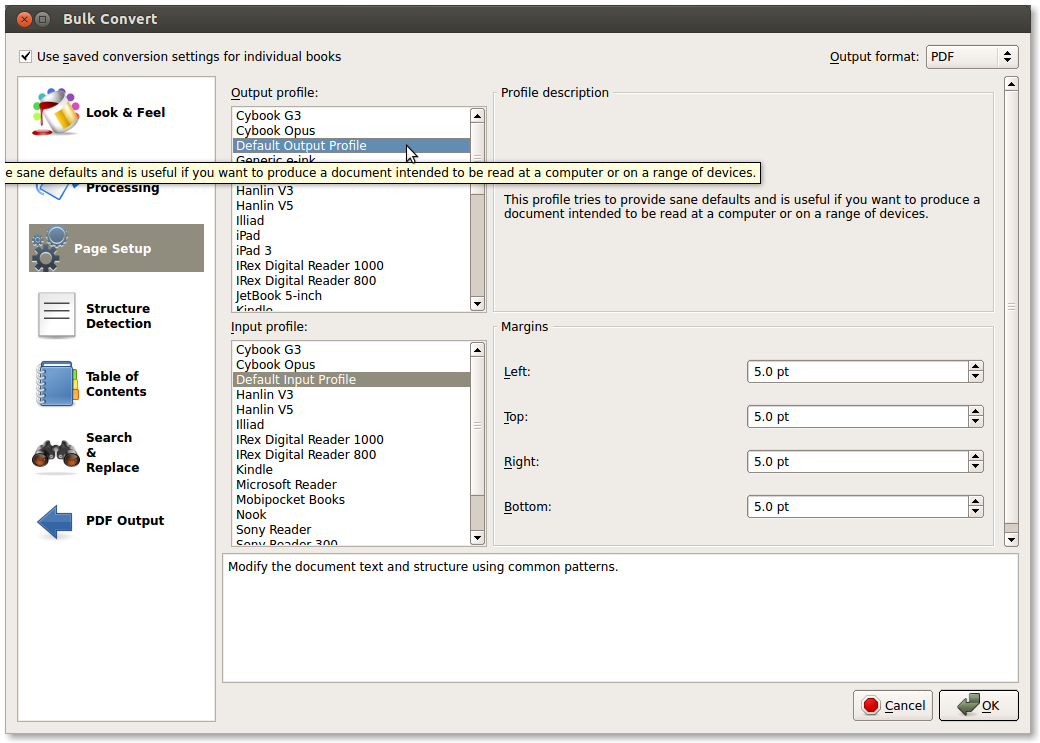
\includegraphics[width=\paperwidth]{graphic/choose_default.png}
\end{frame}


\begin{frame}
\frametitle{Beberapa yang perlu di ingat}
\begin{itemize}
\item Pengubahan setting lain dapat mengubah hasil pilihan output profile 
\item Output profile bawaan calibre adalah 'e-ink device' 
\item Pilih 'Default output profile' terakhir sebelum mengklik 'ok'
\end{itemize}
\end{frame}
 
 
\begin{frame}[shrink=20]
\frametitle{Contoh halaman yang terpotong hasil keluaran dengan profile 'e-ink device'}
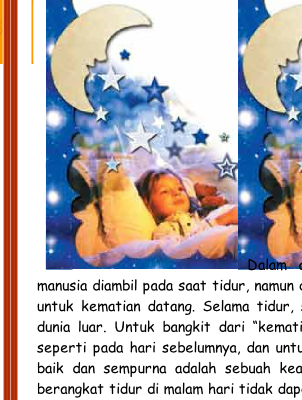
\includegraphics[width=\paperwidth]{graphic/eink_output.png}
\end{frame}


\end{document}
